\chapter{ISTTOK }

\section{Machine description}


\begin{figure}[htbp]
	\centering
	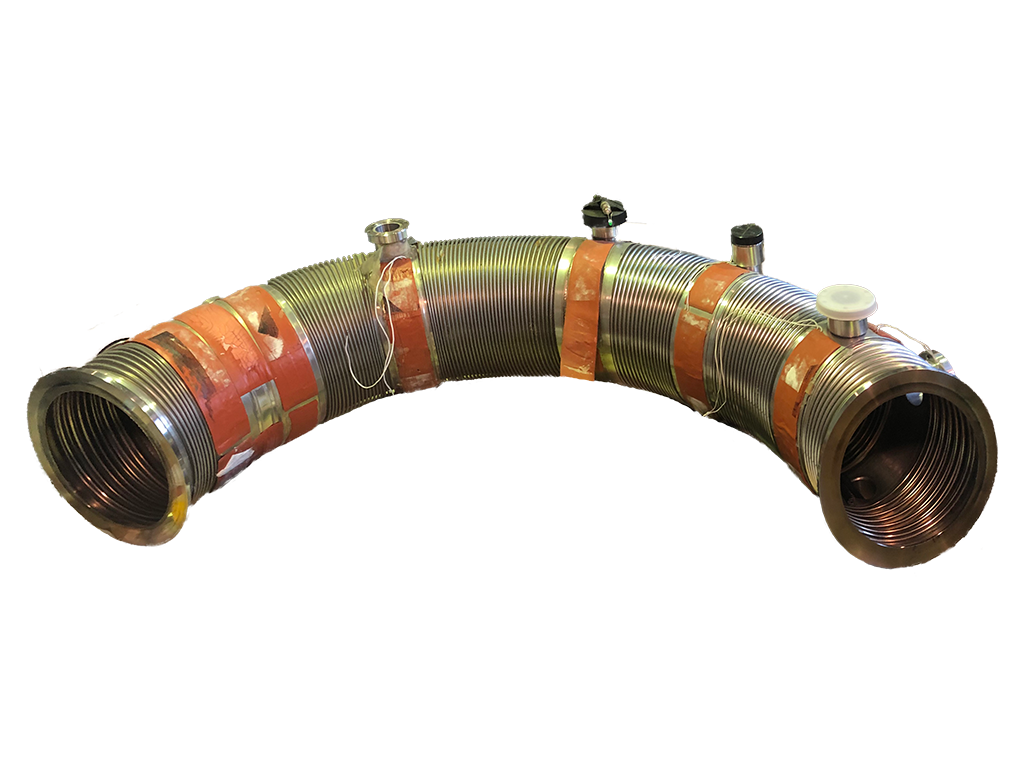
\includegraphics[width=0.65\textwidth]{Chp4/VacuumVessel_Low.png}
	\caption{\label{VV_IST} Actual ISTTOK vaccum vessel section with ports.  }
\end{figure}

\begin{figure}[htbp]
	\centering
	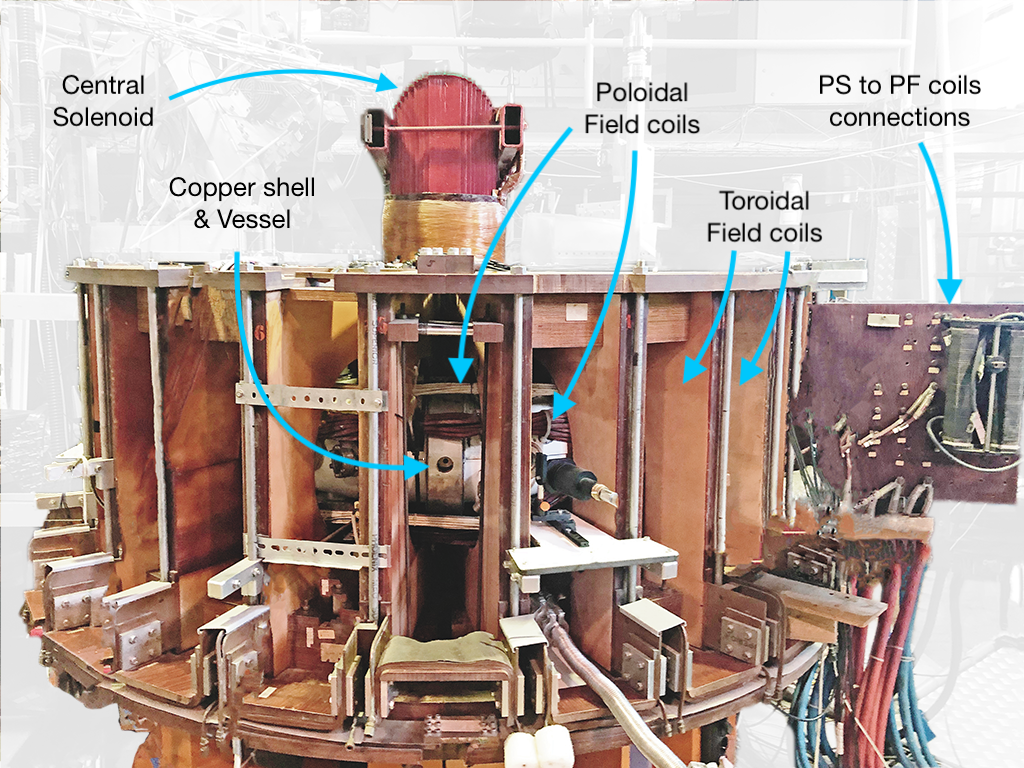
\includegraphics[width=0.765\textwidth]{Chp4/FrontISTTOK.png}
	\caption{\label{ISTTOK_front}ISTTOK frontal view. TF coils.  }
\end{figure}


\section{Diagnostics and Actuators}

\begin{figure}[htbp]
	\centering
	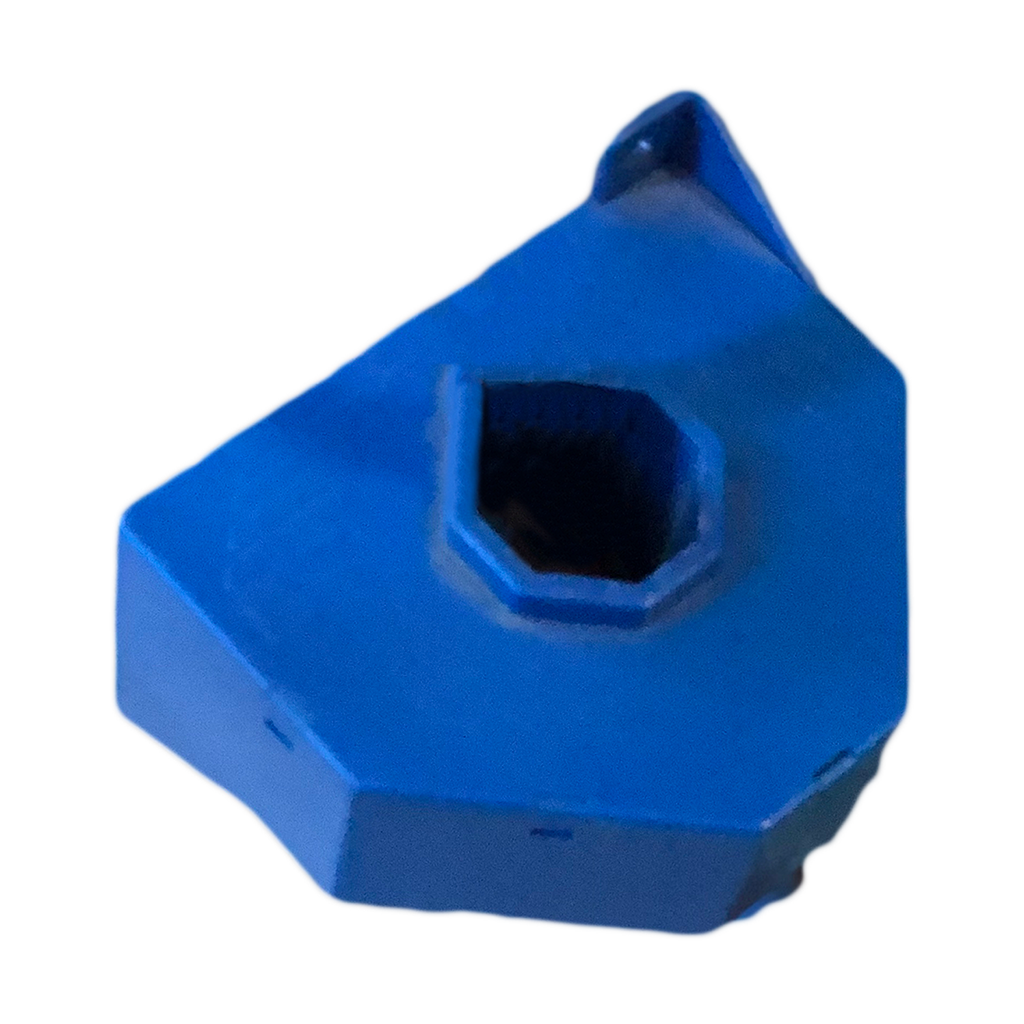
\includegraphics[width=0.465\textwidth]{Chp4/LEM.png}
	\caption{\label{LEM} LEM }
\end{figure}

\begin{figure}[htbp]
	\centering
	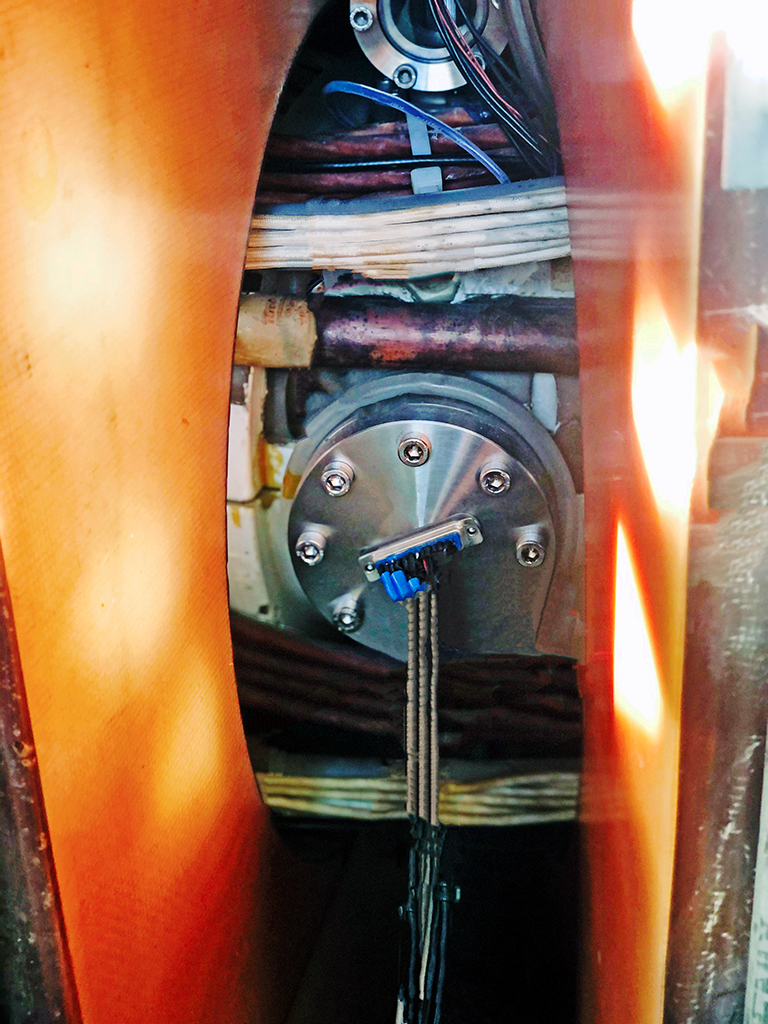
\includegraphics[width=0.465\textwidth]{Chp4/PuertoMirnov.png}
	\caption{\label{MirnPort} Magnetic probes port and PF coils. }
\end{figure}



\section{ATCA-MIMO-ISOL boards}
\subsection{Hardware layout}
\subsection{Real-time  integration software}
\section{Plasma current magnetic field }

Retrieving the contribution of the plasma current in tokamaks ...

The methods of correction of the magnetic error fields due to inaccuracies
of tokamak manufacturing and assembly are considered. The problems of the
plasma position and shape reconstruction based on magnetic field measurements are discussed.

\section{Plasma centroid position determination}